
\setcounter{mtc}{1} %indique le numéro réel du chapitre, pour la mini table des matières
\chapter{Mise en situation}
\minitoc  %insert la minitoc

\graphicspath{{Chapitre1/figures/}}
%==============================================================================
\pagestyle{fancy}
\fancyhf{}
\fancyhead[R]{\bfseries\rightmark}
\fancyfoot[R]{\thepage}
\renewcommand{\headrulewidth}{0.5pt}
\renewcommand{\footrulewidth}{0pt}
\renewcommand{\chaptermark}[1]{\markboth{\MakeUppercase{\chaptername~\thechapter. #1 }}{}}
\renewcommand{\sectionmark}[1]{\markright{\thechapter.\thesection~ #1}}

\begin{spacing}{1.5}

%==============================================================================
\section*{Introduction}
Avant de commencer à détailler le travail réalisé, il est indispensable d'introduire l'organisme d'accueil afin de se faire une idée sur son domaine d'activité, la situation actuelle qui l'a motivé à entreprendre notre projet, ainsi que son orientation.\\
Une fois entamée, nous enchaînerons avec la présentation de la problématique, suivie d'une description sommaire du sujet du projet et des concepts clés associés.\\
La méthodologie employée tout au long de sa mise en oeuvre sera .


%==============================================================================
\section{Présentation de l'organisme d'accueil}
%-----------------------------------------------------------------------------------
\subsection{L'entreprise "IT SERV"}
IT SERV est une société de services et de conseil exerçant dans le domaine des Technologies de l'Information et de la Communication.
Fondée en 2008, elle a très tôt opté pour un positionnement stratégique sur les activités de conseil et de services dans le secteur des TIC en Tunisie. Elle a pour but de fournir des services à forte valeur ajoutée à ses clients. Dans ce cadre, elle vise essentiellement à les orienter vers l'adoption des technologies modernes, à maximiser l'efficacité et l'efficience de leur organisation et à optimiser leurs processus.\\
Ses valeurs fondamentales s'articulent autour de la satisfaction des clients d'une part et l'épanouissement et l'évolution de ses ingénieurs et consultants d'autre part. La figure \ref{fig:organigramme} présente la hiérarchie générale de l'entreprise.\\

\begin{figure}[h]
\centering
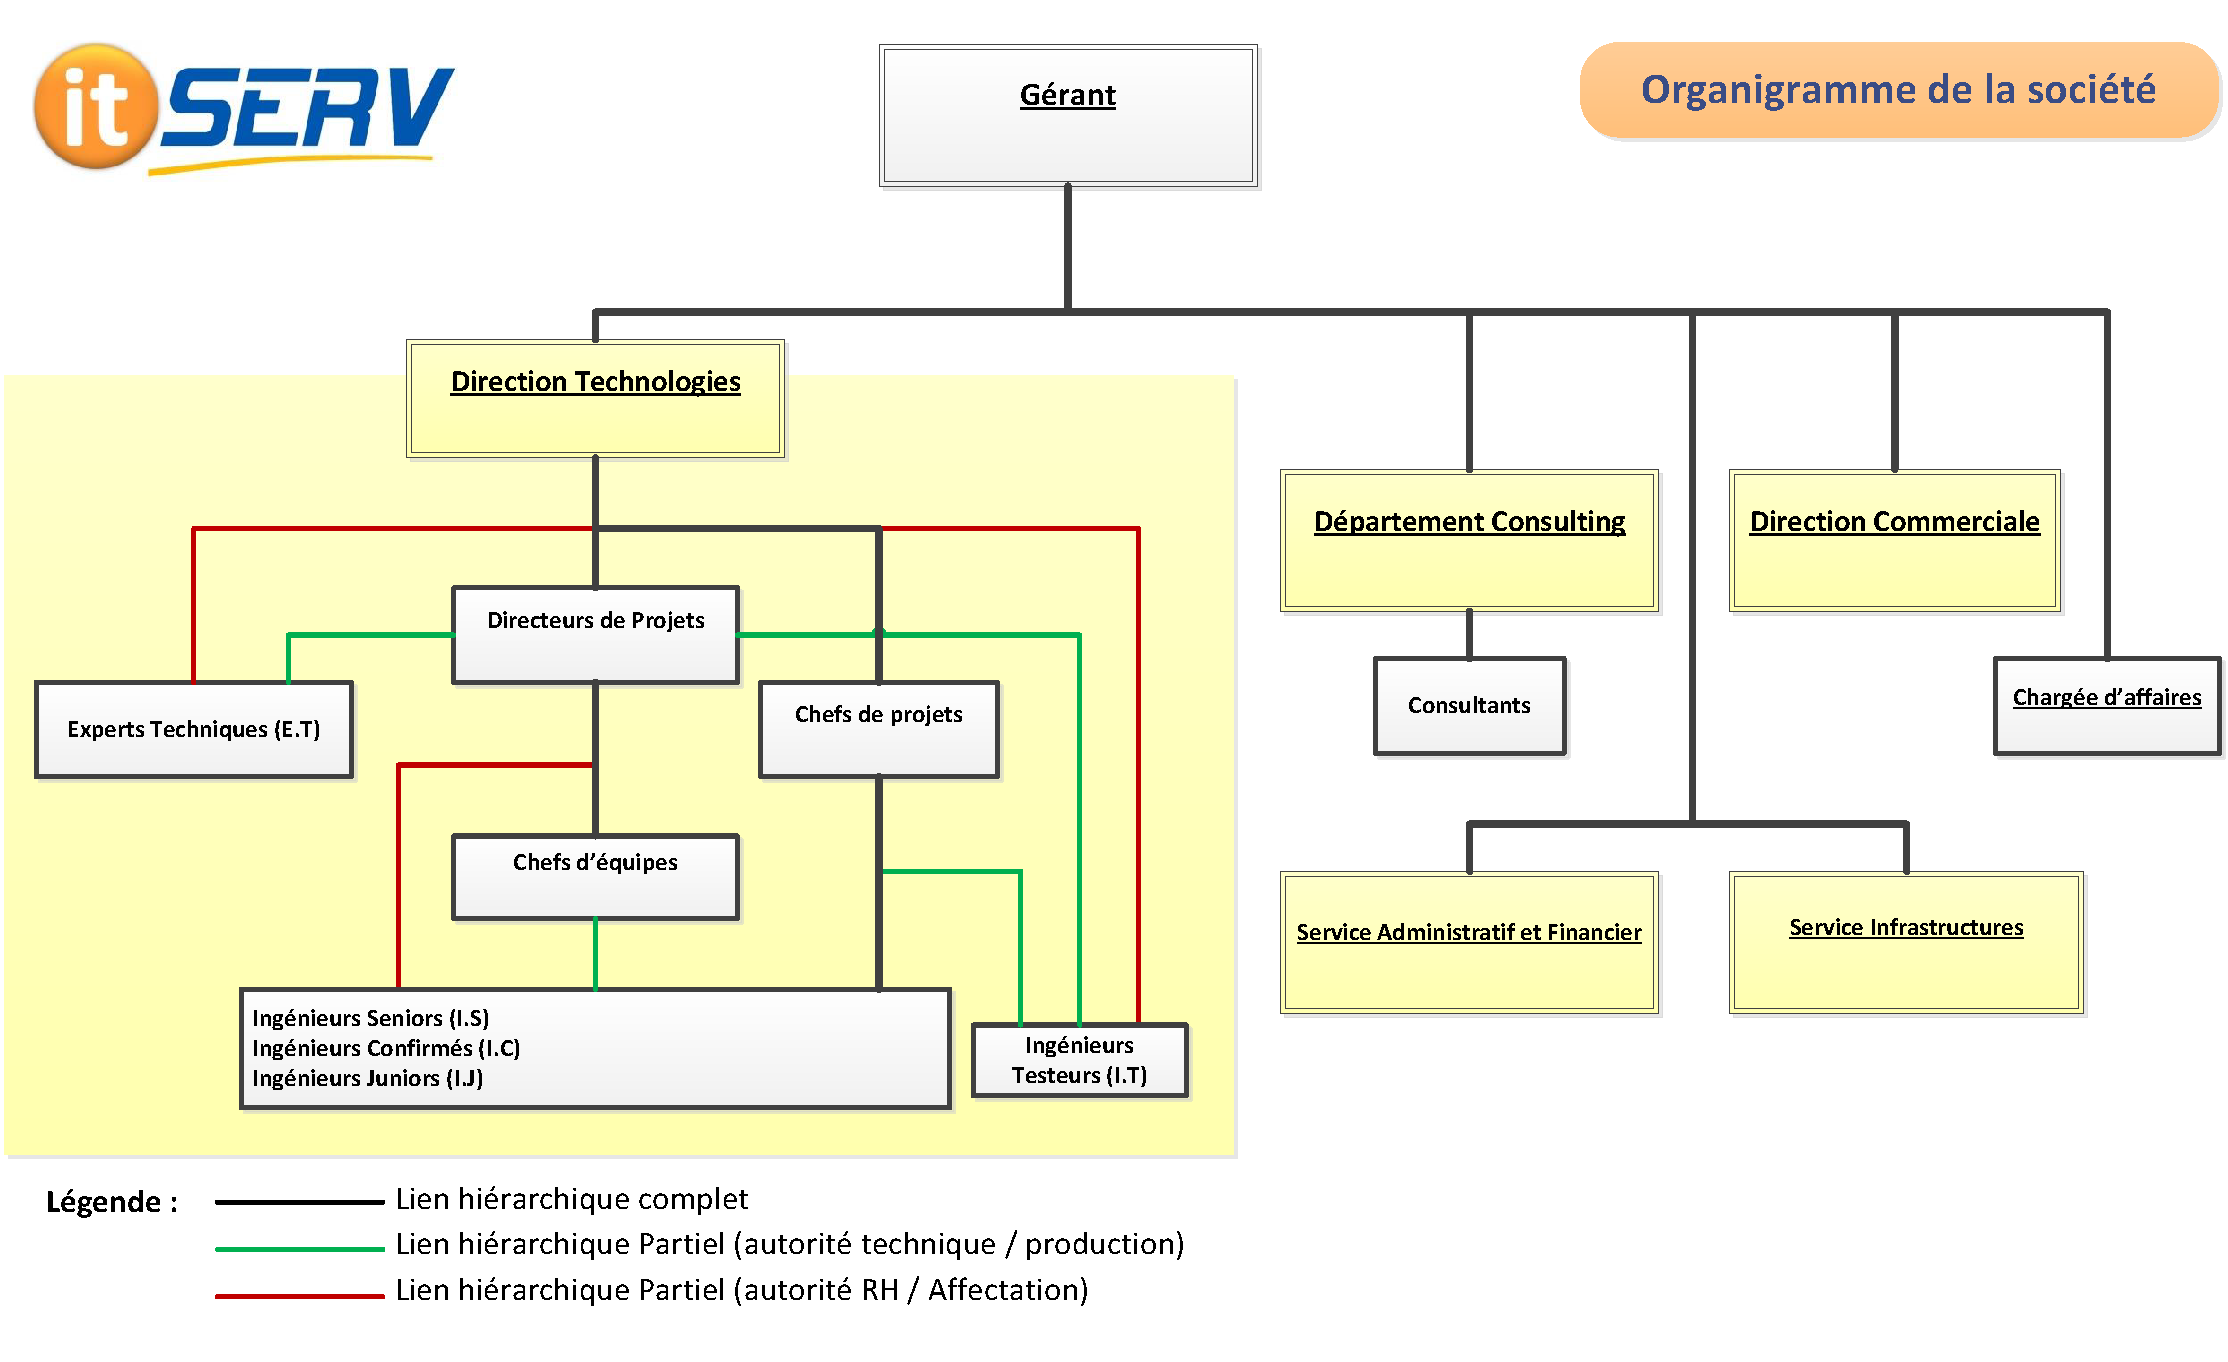
\includegraphics[scale=0.8]{organigramme.png}
\caption{Organigramme de l'entreprise}
\label{fig:organigramme}
\end{figure}

En plein essor, l'entreprise jouit d'une forte croissance sur tous les plans : chiffre d'affaires, résultats, effectifs, périmètre de compétence, portefeuille clients, etc. Cette réussite, à la fois en local et à l'international, constitue un facteur de stabilité et un facteur de confiance en soi pour ses clients et ses collaborateurs. Les graphiques de la figure \ref{statistiquesCroissance} fournissent plus de détail sur l'état actuel des lieux.\\

\begin{figure}[h]
\centering
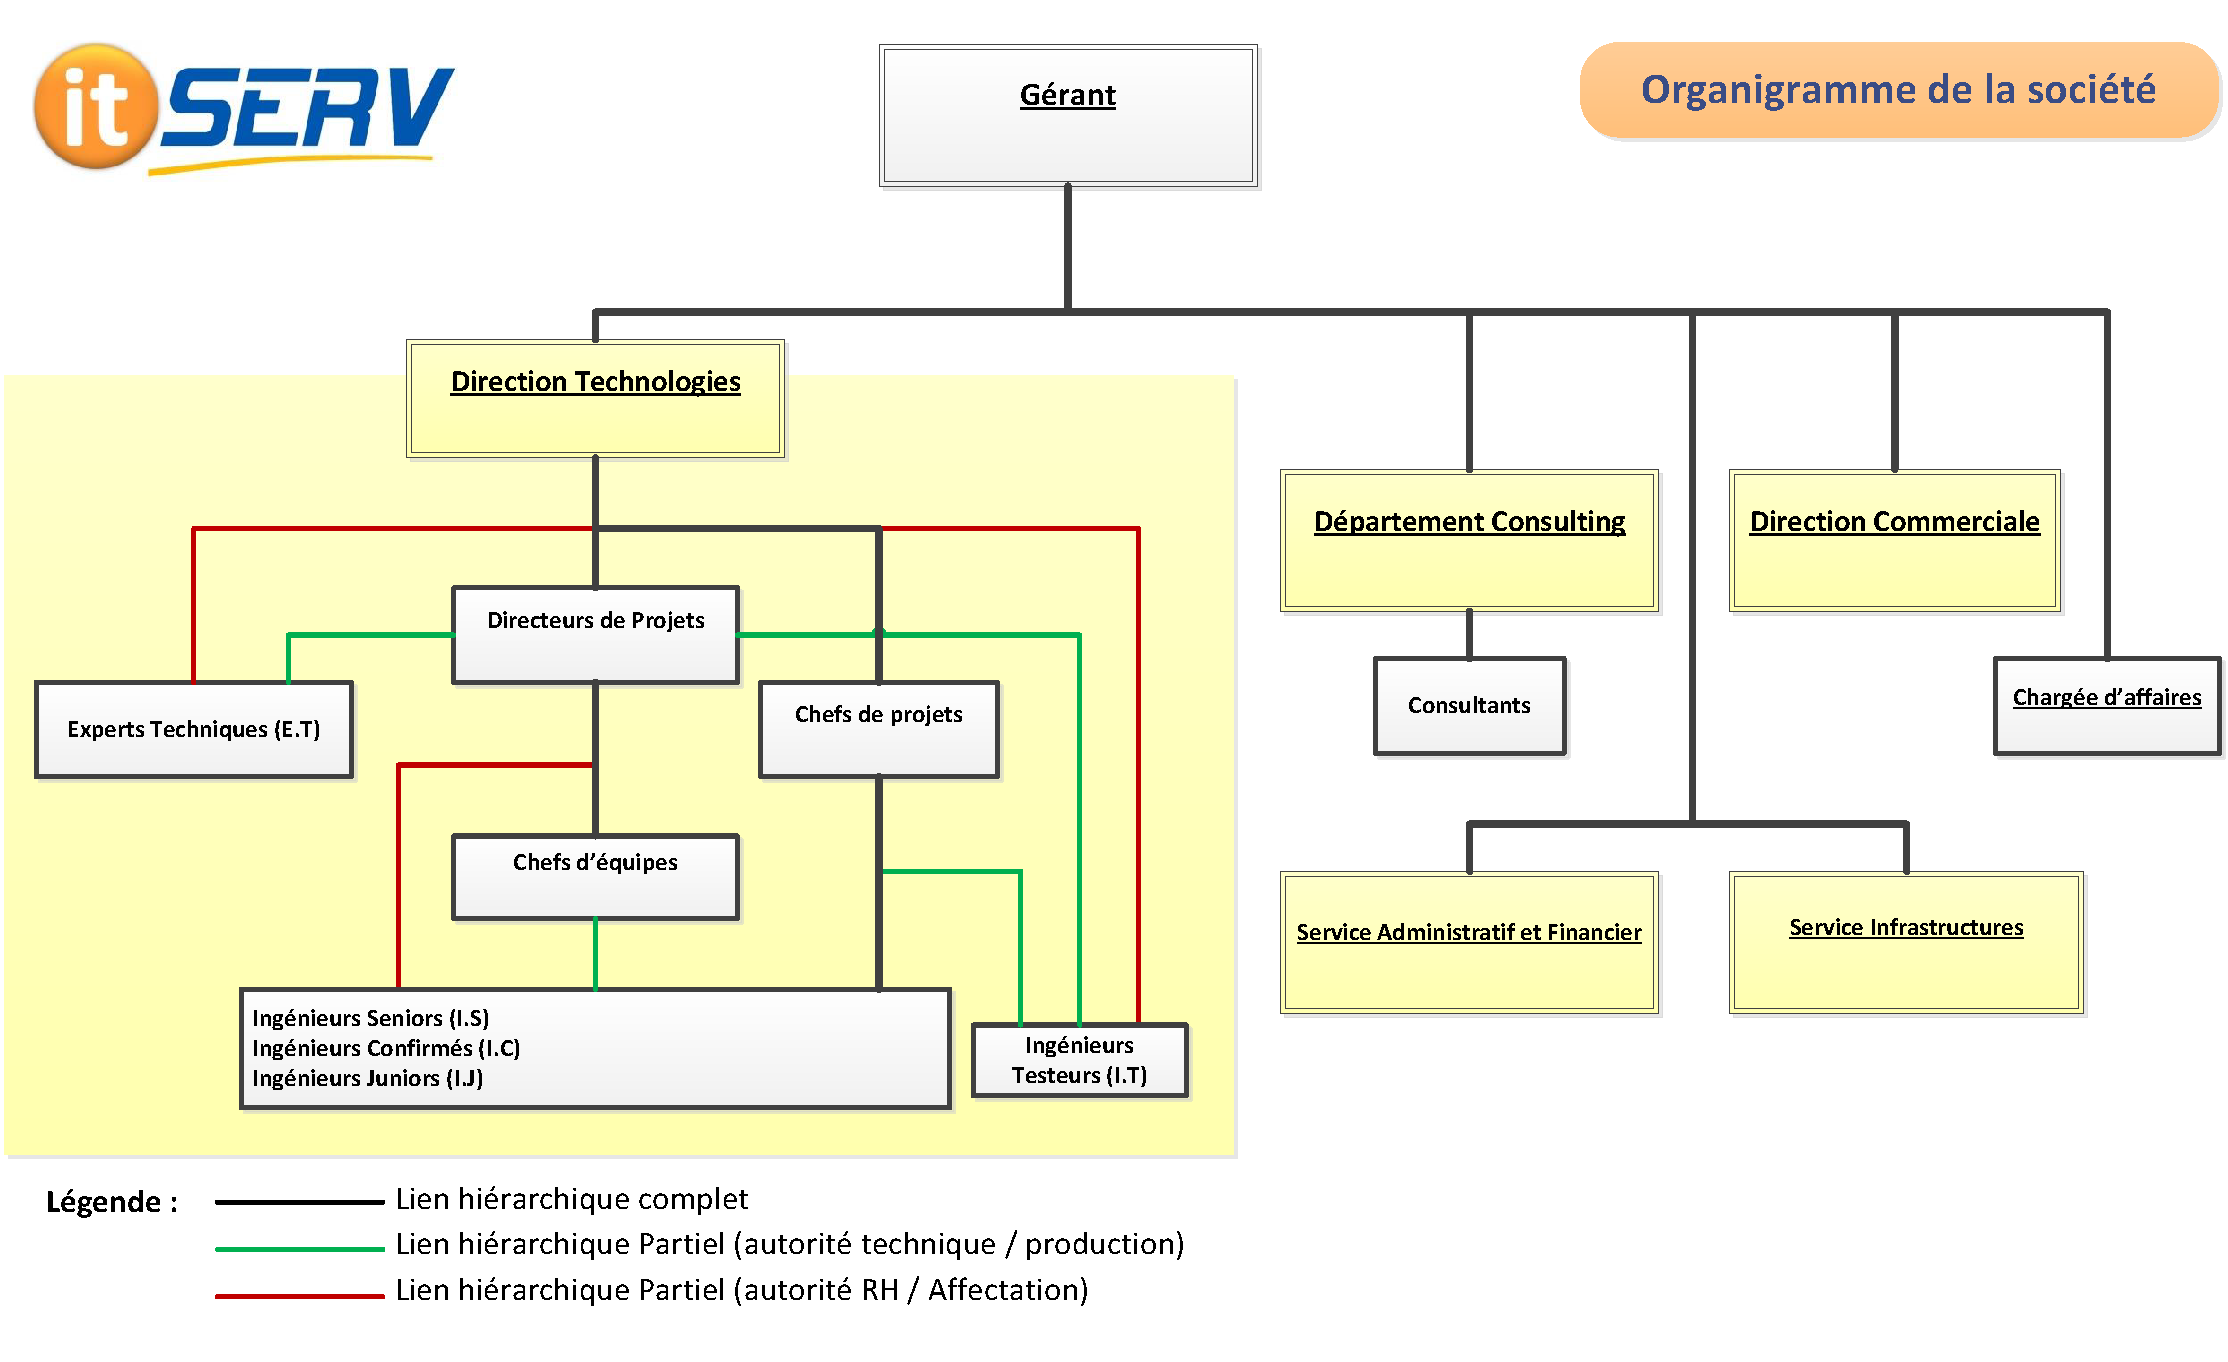
\includegraphics[scale=0.8]{organigramme.png}
\caption{Chiffre d'affaires, Croissance en nombres, Statistiques...}
\label{statistiquesCroissance}
\end{figure}

IT SERV favorise les partenariats s'inscrivant dans la continuité et la durée. En effet elle établit avec la majorité de ses clients des accords cadre, leur permettant de profiter de prix étudiés et de conditions avantageuses en matière de disponibilité, de priorité et d'engagement au plus haut niveau. Cette démarche stratégique lui permet d'avoir en contrepartie une visibilité long terme sur les commandes et les projets de ses clients, de dimensionner ses équipes en conséquence et d'optimiser son investissement en formation et mise à niveau de ses cadres en recherche & développement.

%-----------------------------------------------------------------------------------
\subsection{Domaine d'expertise}
\\\\
Les prestations d'IT SERV s'articulent autour de quatre offres :
\begin{itemize}
    \item Consulting IT
    \item Intégration \& Développement
    \item Expertise Télécoms
    \item Nearshore Outsourcing
\end{itemize}
\\\\
L'entreprise vise la réalisation de missions complexes ayant un apport conséquent pour ses clients, dans un cadre de partenariat bénéfique pour les deux parties. La réussite de toutes ses missions et l'atteinte des objectifs ont instauré des relations de confiance très durables et un élargissement progressif du périmètre d'intervention.

\begin{figure}[!ht]
\centering
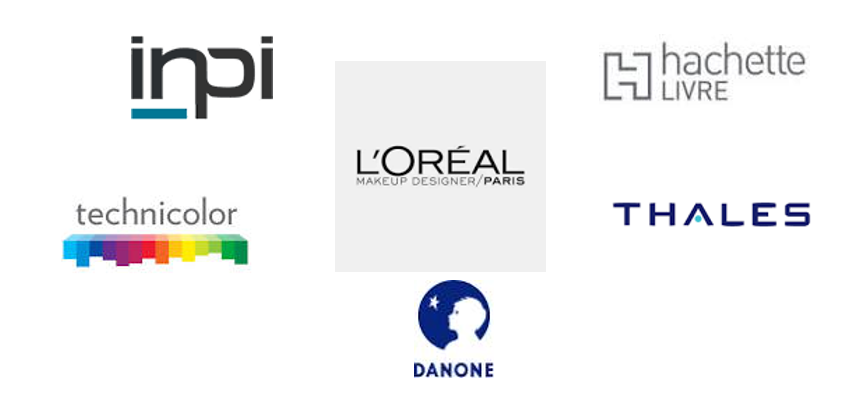
\includegraphics[scale=0.8]{reference.png}
\caption{Références de l'entreprise}
\label{refenrences}
\end{figure}

Plus récemment, l'entreprise aspire à élargir son éventail d'offres et entrevoit de se convertir en un éditeur de logiciel à part entière.


%==============================================================================
\section{Problématiques et motivations}
De nos jours, la gestion de projet s'impose dans les structures de toutes tailles comme le mode d'organisation par excellence.\\
Un projet désigne un ensemble finalisé d'activités et d'actions entreprises dans le but de répondre à un besoin, soumis à des contraintes bien définies, généralement dans des délais fixés avec une allocation budgétaire plafonnée. La gestion de projet quant à elle, représente la démarche visant à organiser de bout en bout le bon déroulement d'un projet.\\
Celle-ci revient généralement à la gestion de multiples facettes, notamment :
\begin{itemize}
    \item La planification
    \item La gestion budgétaire
    \item Le pilotage des risques
    \item La gestion du changement
    \item La gestion des interventions
    \item La gestion des mises à jour
    \item La gestion des ressources
\end{itemize}
\

Avec les projets de plus en plus complexes auquels les entreprises font face, gérer tous les flux d'information en perpétuel changement d'un projet se révèle être une tâche des plus ardues pour les chefs de projets. Sans un système efficace de traitement des données et d'achemeninement de l'information, ceux-ci finissent par être submergés par les requêtes, et se retrouvent le plus souvent dépassés par les événements. Ceci se reflète en conséquence par un manquement au niveau de la réponse aux attentes de l'une ou plusieurs des parties prenantes au projet, qui, souvent dû à des contraintes de disponibilité, restent trop longtemps en déphasage avec les dernières fluctuations et les mises à jour du projet.\\
C'est là que réside le coeur de la problématique : réussir à synchroniser de manière efficace toutes les parties prenantes à un projet avec l'état actuel de ce dernier, en distinguant le chef de projet en tant que pièce maîtresse de sa supervision.\\
\\
Le projet présent a pour but de répondre à ce problème en fournissant une solution logicielle dédiée à la gestion de projets. La solution se doit de répondre adéquatement aux attentes des chefs de projets en termes de fonctionnalités, mais aussi fournir un point pivotal d'aide à la décision pour les dirigeants de l'entreprise. En effet, les données récupérées tout au long de son exercice devront être en mesure d'être synthétisées en des données actionables, capables d'orienter les dirigeants de l'entreprise dans leur prise de décisions stratégiques quant à la détermination des clients les plus profitables, les partenariats les plus importants, etc.\\
Au sein de l'environnement extrêmement concurrentiel dans lequel exerce l'entreprise, et au vu du poids dont relève sa prestation de consulting en termes de gestion de bout en bout de projets, il est clair qu'une solution dédidée à la gestion du portefeuille de projets de l'entreprise avec ses clients constituerais un point fort face à la concurrence et impacterais positivement l'image de la société en influençant grandement le niveau de satisfaction de ses clients.\\
\\
Outre l'apport de l'application pour la gestion de ses propres projets en interne, dans l'optique de sa conversion en un éditeur de logiciel, IT SERV entrevoit de développer une offre autour d'une version SaaS de l'application.\\
 Dans ce cadre, le développement d'une interface de gestion et de monitoring de l'aspect SaaS de l'application s'impose en tant que partie à part entière du projet. Elle se verras traîtée plus en détail au cours du chapitre \ref{chapterX}.


%==============================================================================
\section{Méthodologie de travail}
%-----------------------------------------------------------------------------------
\subsection{Le choix de la méthodologie}
La grande ?volution dans le domaine du d'veloppement est accompagn?e par une ?volution des moyens assurant le bon fonctionnement de ce dernier. D'o? l'apparition des m?thodes agiles permettant d'organiser le cycle de d'veloppement des projets informatiques.

Les m?thodes agiles sont bas?es sur des principes communs d'finis dans l'Agile Manifesto qui est r?dig? par des experts dans ce domaine \cite{AgManifesto}. Ils se reposent essentiellement sur une approche it?rative incr?mentale et adaptative ?voluant en parall?le avec les besoins du client, afin de livrer un produit de qualit?.
Il existe plusieurs m?thodes agiles, ? savoir, la m?thode  RUP \cite{RUP}, la m?thode XP \cite{XP}, la m?thode SCRUM \cite{SCRUM} et la m?thode RAD \cite{RAD}.

%-----------------------------------------------------------------------------------
\subsection{La méthodologie DAD}
Dans la majorit? des projets, il est difficile d'anticiper les attentes du client. Ceci nous oriente vers une approche it?rative permettant de s'adapter aux exigences du client au fur et ? mesure de l'avancement du projet. Pour ce faire, nous avons choisi d'adopter la m?thode Scrum.
Aujourd'hui, Scrum est la m?thode agile la plus utilis?e. Elle permet de produire une solution de la plus haute qualit? dans des bref d'lais.
Cette m?thode est munie des atouts suivants :
\begin{itemize}
  \item Meilleur vue d'ensemble du projet : nous avons une vue globale sur l'avancement du projet par tous les membres des diff?rentes ?quipes avec un traitement r?gulier des probl?mes rencontr?s durant chaque phase.
  \item Mise ? jour des priorit?s : le client, qui n'est pas n?cessairement un informaticien, n'a pas toujours une vision compl?te sur le produit final. Pour cela, et gr?ce ? la composition s?quentielle du contenu des sprints, il b?n?ficie d'une flexibilit? au niveau de la d'finition, de l'?volution des priorit?s et des s?quences d'activit?s.
  \item Qualit? du produit mise en avant : Cette m?thode se repose sur une ?valuation r?guli?re du travail, ce qui permet un meilleur traitement des probl?mes (bug), une meilleure productivit? et un produit satisfaisant \cite{AvantageScrum}.
\end{itemize}

Notion :
\begin{itemize}
  \item Sprint  : une it?ration de travail qui dure entre 15 et 30 jours.
  \item Le product backlog : repr?sente la liste des fonctionnalit?s r?dig?es par le product owner avec tous les correctifs et les am?liorations. Il est donc modifiable tout au long du projet. Le product backlog est pr?sent? sous forme d'items.
  \item Le sprint backlog : est l'ensemble des items planifi?s pour le sprint en cour \cite{SCRUM}.
\end{itemize}


%==============================================================================
\section*{Conclusion}
Dans ce chapitre, nous avons pr?sent? le cadre g?n?ral du travail, en commen?ant par la pr?sentation de l'entreprise Urbaprod, passant par la probl?matique du projet, ainsi qu'une ?tude des solutions existantes sur le march?. Et pour finir, nous avons pr?sent? la m?thode qui va guider notre travail tout au long du projet. Dans le chapitre suivant, nous introduisons les sp?cifications de notre projet.


%==============================================================================
\end{spacing}
